\chapter{Object analysis}

\FloatBarrier

\section{Description of the subject area}

A supermarket inventory system relates identifiable products to the quantities available for store operations. Goods arrive through deliveries and leave through sales, transfers, damage and other dispatches, while physical counts produce observations that may disagree with the recorded balance. Even though Shelfwise neither executes sales nor places orders with suppliers, it must represent the stock effect of both. The subject of this thesis is this inventory workflow within a single store.


The current balance and the movement history answer different questions. The balance answers a short operational one—how much of this product is recorded now?—whereas the history answers a longer explanatory one: which accepted changes produced that balance? A system that keeps only the balance cannot recover an omitted reason or tell a double submission from two genuine deliveries. A system that keeps only events can explain every change but needs extra work to serve fast, filtered inventory pages. Shelfwise therefore stores the balance together with its accepted movement records.


Each product carries descriptive context: identity, category, supplier, unit and current price. The SKU is a required unique identifier and the barcode is optional. Stock received through a purchase may also carry a batch number, production date and expiry date. The unit label always describes a whole-number quantity, so a label such as kg does not add decimal weighing; a weighing workflow would require fractional units and an explicit rounding policy. Sellable quantity excludes expired and quarantined batches, whereas physical quantity still includes them for disposal and reconciliation.


Inventory value is a presentation estimate: the current physical quantity of each active product multiplied by its current unit price. It is neither supplier cost, historical cost of goods sold nor an accounting valuation, and keeping this distinction prevents a convenient dashboard figure from being read as financial evidence. Likewise, the store currency preference changes only the displayed currency code and symbol and does not convert stored prices.


\FloatBarrier

\section{Operational problems and system boundary}

Manual stock work fails in several distinct ways. A delivery may be entered twice after a slow response; two dispatches may each rely on an outdated balance; a correction may be entered as a relative change when the employee meant an absolute count; and a manager may acknowledge a warning while the item is still out of stock. Because these are different problems, their controls must preserve their meanings instead of reducing every case to a generic update.


The system boundary covers product and reference-data administration, searchable inventory, receiving, dispatch, adjustment, stocktake, batch control, expiry and slow-moving warnings, warning review, replenishment suggestions, purchase drafting and approval, partial receipts, count and disposal reviews, reports and staff access. It excludes payment processing, supplier invoicing, checkout integration, customer reservations and multiple stores. A supplier record remains purely descriptive until a purchase document refers to it, and a purchase document affects stock only once a receipt is accepted.


The case study uses fictitious supermarket records and a local deployment. Its evaluation covers transaction correctness, request authorization, warning behavior and selected performance and recovery scenarios; effects on shelf availability or employee productivity would require evaluation with store staff and operational data. Table~\ref{tab:scope} summarizes the resulting boundary.


\begin{table}[htbp]\centering\small\setstretch{1.05}\setlength{\tabcolsep}{3pt}\renewcommand{\arraystretch}{1.25}
\caption{Implemented domain and excluded extensions}\label{tab:scope}
\begin{tabular}{>{\raggedright\arraybackslash}p{0.3\textwidth}>{\raggedright\arraybackslash}p{0.3\textwidth}>{\raggedright\arraybackslash}p{0.3\textwidth}}
\toprule
\textbf{Aspect} & \textbf{Implemented meaning} & \textbf{Extension outside the current boundary} \\
\midrule
\leavevmode{}Store organization & \leavevmode{}One shared store workspace & \leavevmode{}Tenant and branch isolation \\
\leavevmode{}Quantity & \leavevmode{}Bounded integer balance & \leavevmode{}Decimal weights and unit conversion \\
\leavevmode{}Stock operation & \leavevmode{}Receive, dispatch, adjust and count, with batch-aware receipt and dispatch & \leavevmode{}Checkout and reserved stock \\
\leavevmode{}Supplier & \leavevmode{}Product partner, replenishment suggestion and purchase workflow & \leavevmode{}Invoices and settlement \\
\leavevmode{}Warning & \leavevmode{}Quantity, expiry, slow-moving and recovery episodes with review & \leavevmode{}Demand forecasting and automatic purchasing \\
\leavevmode{}Financial display & \leavevmode{}Current price multiplied by physical quantity as a presentation estimate & \leavevmode{}Accounting cost and profit \\
\leavevmode{}Phone access & \leavevmode{}Responsive browser interface & \leavevmode{}Native Android or iOS application \\
\bottomrule\end{tabular}\end{table}

\FloatBarrier

\section{Construction of the conceptual model}

The functional model in Figure~\ref{fig:functions} divides the system into seven modules: identity and access, catalog, stock activity, batches and reviews, warnings, purchasing and reporting. The modules carry different responsibilities but share the product identity. Catalog work defines what a product is and how it is classified; stock activity changes its bounded quantity; batches and reviews track dated stock and approve corrections; warnings interpret the quantity against policy and record review; purchasing turns shortages into approved orders and receipts; and reporting summarizes the accepted facts.


\begin{figure}[htbp]\centering
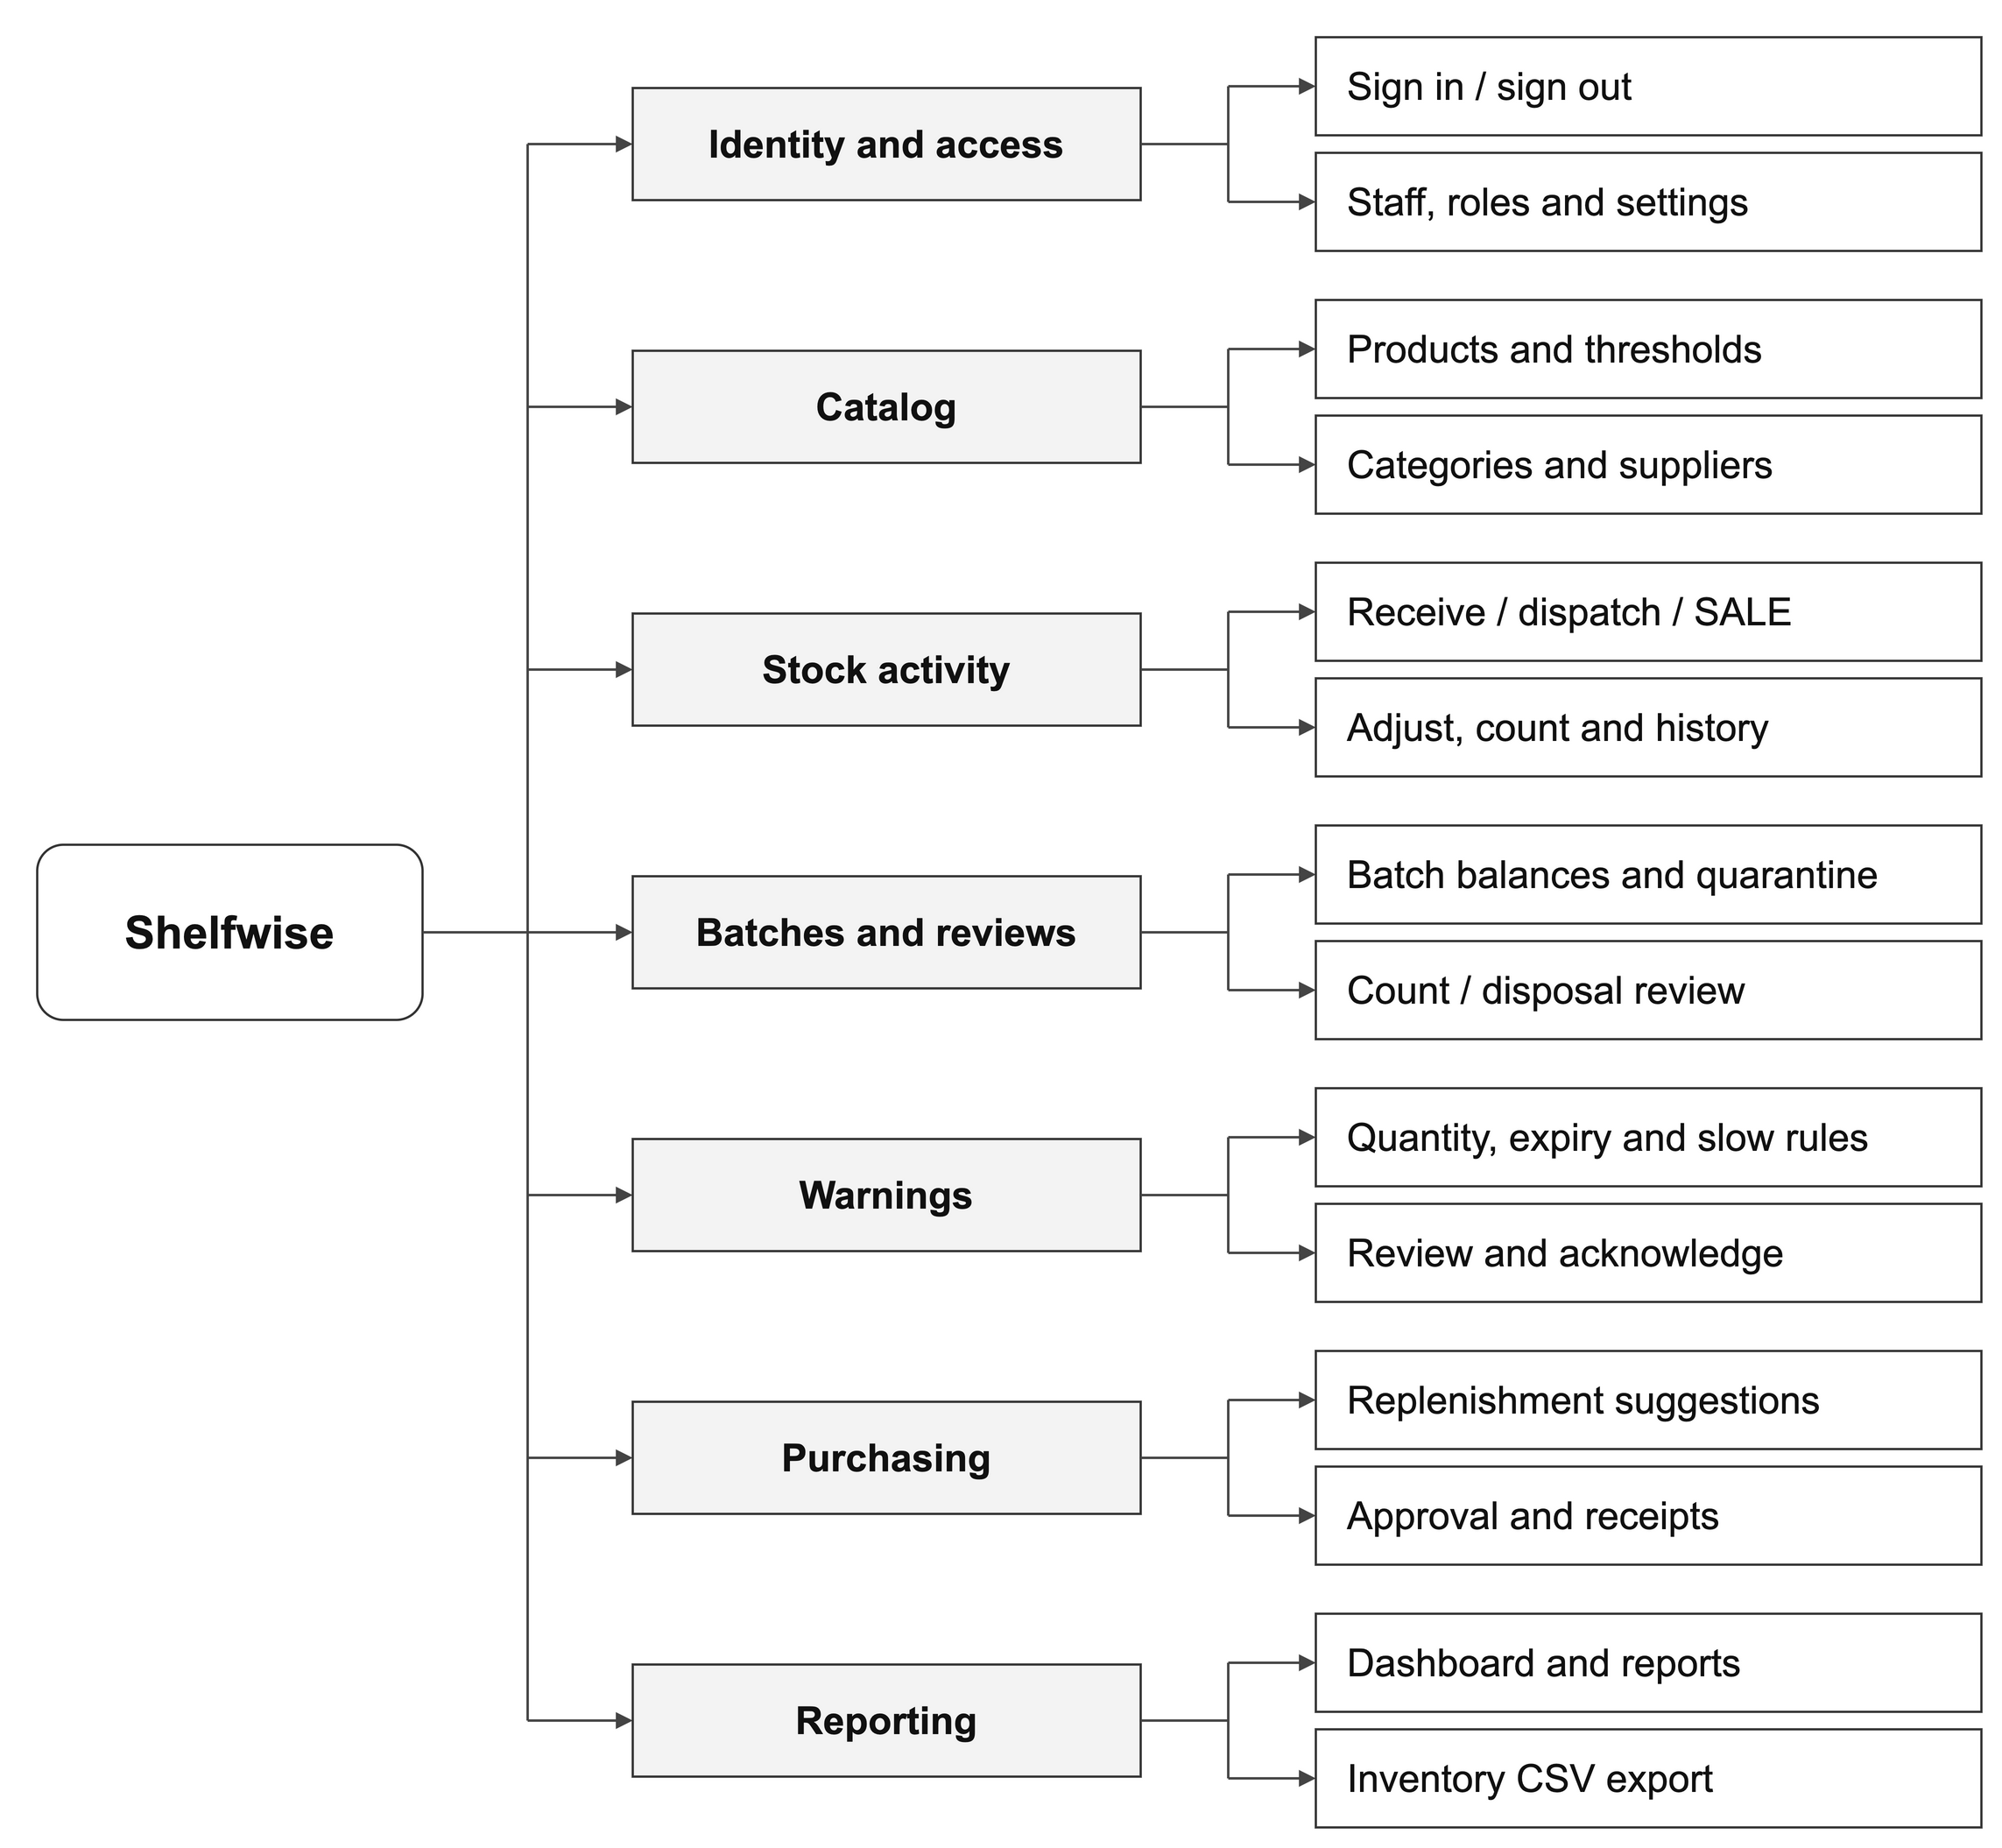
\includegraphics[width=\textwidth,height=0.70\textheight,keepaspectratio]{../figure-assets/diagrams/01-functional-model.png}
\caption{Overall functional model of the supermarket inventory system}\label{fig:functions}
\end{figure}

The division is most useful when a requirement spans several modules. Receiving stock, for example, changes a product, creates a movement, may resolve a shortage and alters dashboard totals. Separate responsibilities do not imply separate services, and Chapter 3 explains why these effects are coordinated within a single database transaction.


\subsection{Product catalog model}

A product has a SKU, an optional barcode, a name, a unit, a current price, a category and an optional supplier. Its stock policy consists of a safety stock and a reorder threshold. The current quantity is displayed alongside the product but cannot be entered in the catalog; it changes only through an inventory operation. An archived product keeps its identity and history but rejects further stock movements.


Authority over the catalog differs from authority over stock. Administrators manage product identity and archival, managers inspect inventory and update thresholds, and clerks consult product information before posting stock; the role matrix in Chapter 3 records the exact boundaries.


Categories organize the inventory view and its totals, and suppliers hold descriptive partner information that may be linked to products. Neither reference type owns a stock balance. Deleting a category or supplier that is still referenced violates its foreign-key relationship, so stock-bearing records follow the separate archival lifecycle instead.


\subsection{Stock activity model}

Shelfwise records five movement types, summarized in Table~\ref{tab:movements}. STOCK\_IN takes a positive quantity and increases stock. STOCK\_OUT and the manually recorded SALE also take positive quantities but decrease stock; only SALE counts as a sale for slow-moving detection, and it records the stock effect of a sale without any checkout or payment integration. ADJUSTMENT takes a signed, non-zero change. STOCKTAKE supplies an absolute observed quantity, from which the server derives the delta under the product lock. Every accepted record keeps the actual before quantity, the signed delta and the after quantity.


\begin{table}[htbp]\centering\small\setstretch{1.05}\setlength{\tabcolsep}{3pt}\renewcommand{\arraystretch}{1.25}
\caption{Meaning of stock input and resulting change}\label{tab:movements}
\begin{tabular}{>{\raggedright\arraybackslash}p{0.225\textwidth}>{\raggedright\arraybackslash}p{0.225\textwidth}>{\raggedright\arraybackslash}p{0.225\textwidth}>{\raggedright\arraybackslash}p{0.225\textwidth}}
\toprule
\textbf{Movement type} & \textbf{Meaning of entered quantity} & \textbf{Derived delta} & \textbf{Operational example} \\
\midrule
\leavevmode{}\allowbreak{}\path|STOCK_IN|\allowbreak{}\allowbreak{} & \leavevmode{}Positive amount received & \leavevmode{}Positive entered amount & \leavevmode{}Morning delivery \\
\leavevmode{}\allowbreak{}\path|STOCK_OUT|\allowbreak{}\allowbreak{} & \leavevmode{}Positive amount dispatched & \leavevmode{}Negative entered amount & \leavevmode{}Goods leaving the stockroom \\
\leavevmode{}SALE & \leavevmode{}Positive amount sold & \leavevmode{}Negative entered amount & \leavevmode{}Manually recorded sale without checkout \\
\leavevmode{}ADJUSTMENT & \leavevmode{}Signed correction & \leavevmode{}Entered signed amount & \leavevmode{}Two damaged units removed \\
\leavevmode{}STOCKTAKE & \leavevmode{}Absolute observed amount & \leavevmode{}Observed amount minus locked balance & \leavevmode{}Weekly physical count \\
\bottomrule\end{tabular}\end{table}

The use cases in Figure~\ref{fig:uc-stock} separate routine stock posting from reviewed corrections. Administrators and clerks receive goods, dispatch them and record SALE movements. Clerks submit adjustments, counts and disposals through the stock-review workflow, and administrators or managers approve them; administrators additionally retain direct ADJUSTMENT and STOCKTAKE access through the API. All three roles can inspect movement history, and the server, not the client, supplies the authenticated actor and the before and after quantities.


\begin{figure}[htbp]\centering
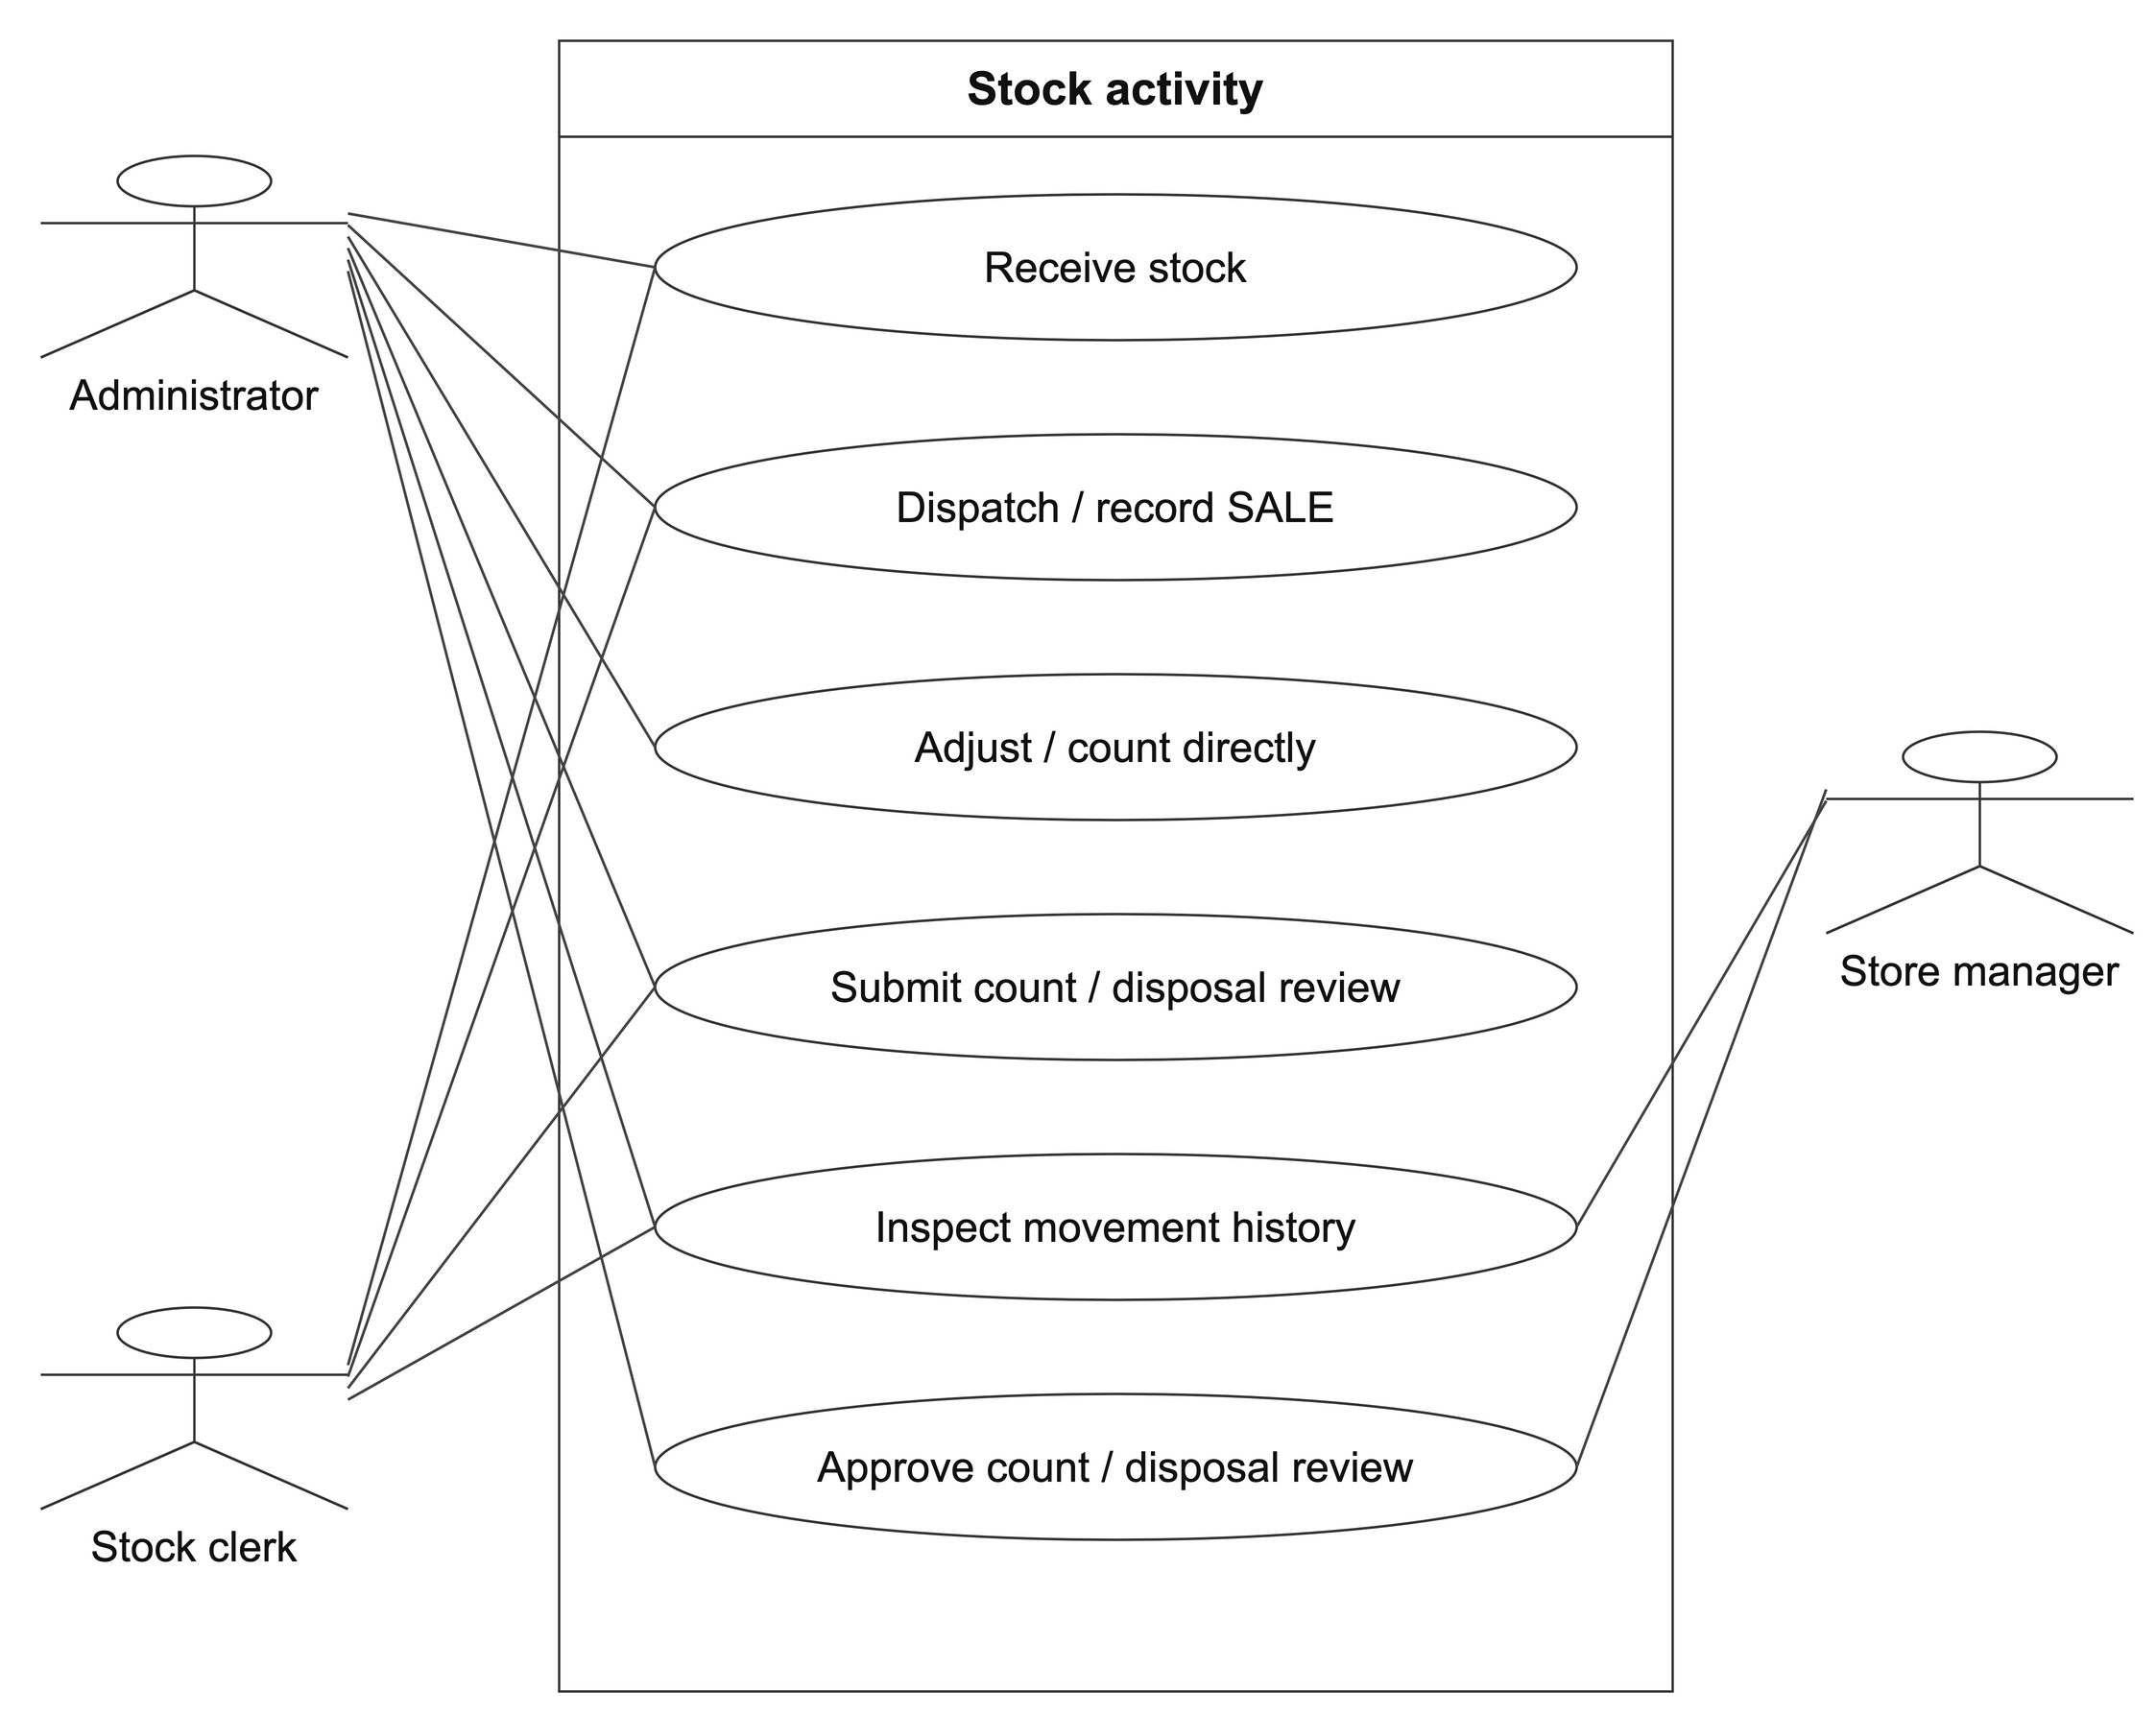
\includegraphics[width=\textwidth,height=0.70\textheight,keepaspectratio]{../figure-assets/diagrams/03-uc-stock.png}
\caption{Stock operation and history use cases}\label{fig:uc-stock}
\end{figure}

Every accepted movement carries a mandatory reason, an actor taken from authentication and a server-assigned timestamp, which together support the investigation of a disputed quantity. A correction is recorded as a further movement, so the earlier record is preserved.


\subsection{Warning and recovery model}

A warning is a persisted episode that links a product to a rule interpretation. OUT and LOW describe sellable quantity, EXPIRING and EXPIRED describe batch dates, SLOW describes a lack of sales over a configured window, and RESTOCKED records a recovery interval. Expiry dates are evaluated in the configured business timezone. A healthy replenishment can resolve a shortage and open a time-limited RESTOCKED episode, and acknowledgement remains independent of all these conditions.


Acknowledgement records a reviewer and a review time; it neither changes the quantity nor resolves the shortage. The distinction matters after a partial replenishment, when a reviewed product may still be LOW and the existing episode keeps its reviewer. A transition from LOW to OUT, or from OUT to LOW, resolves the old episode and opens a new one at the new severity.


Episodes serve both current attention and historical explanation. Open warnings tell a manager what currently needs review, and resolved records show when a shortage or recovery interval ended. The dashboard and warning board are views of these records rather than independent sources of stock truth. Figure~\ref{fig:warning-rules} shows the three rule families and the input each one reads: the quantity rule uses sellable quantity, the expiry rule uses batch dates and the slow-moving rule uses SALE movements only. All three write warning episodes, and none of them changes stock.


\begin{figure}[htbp]\centering
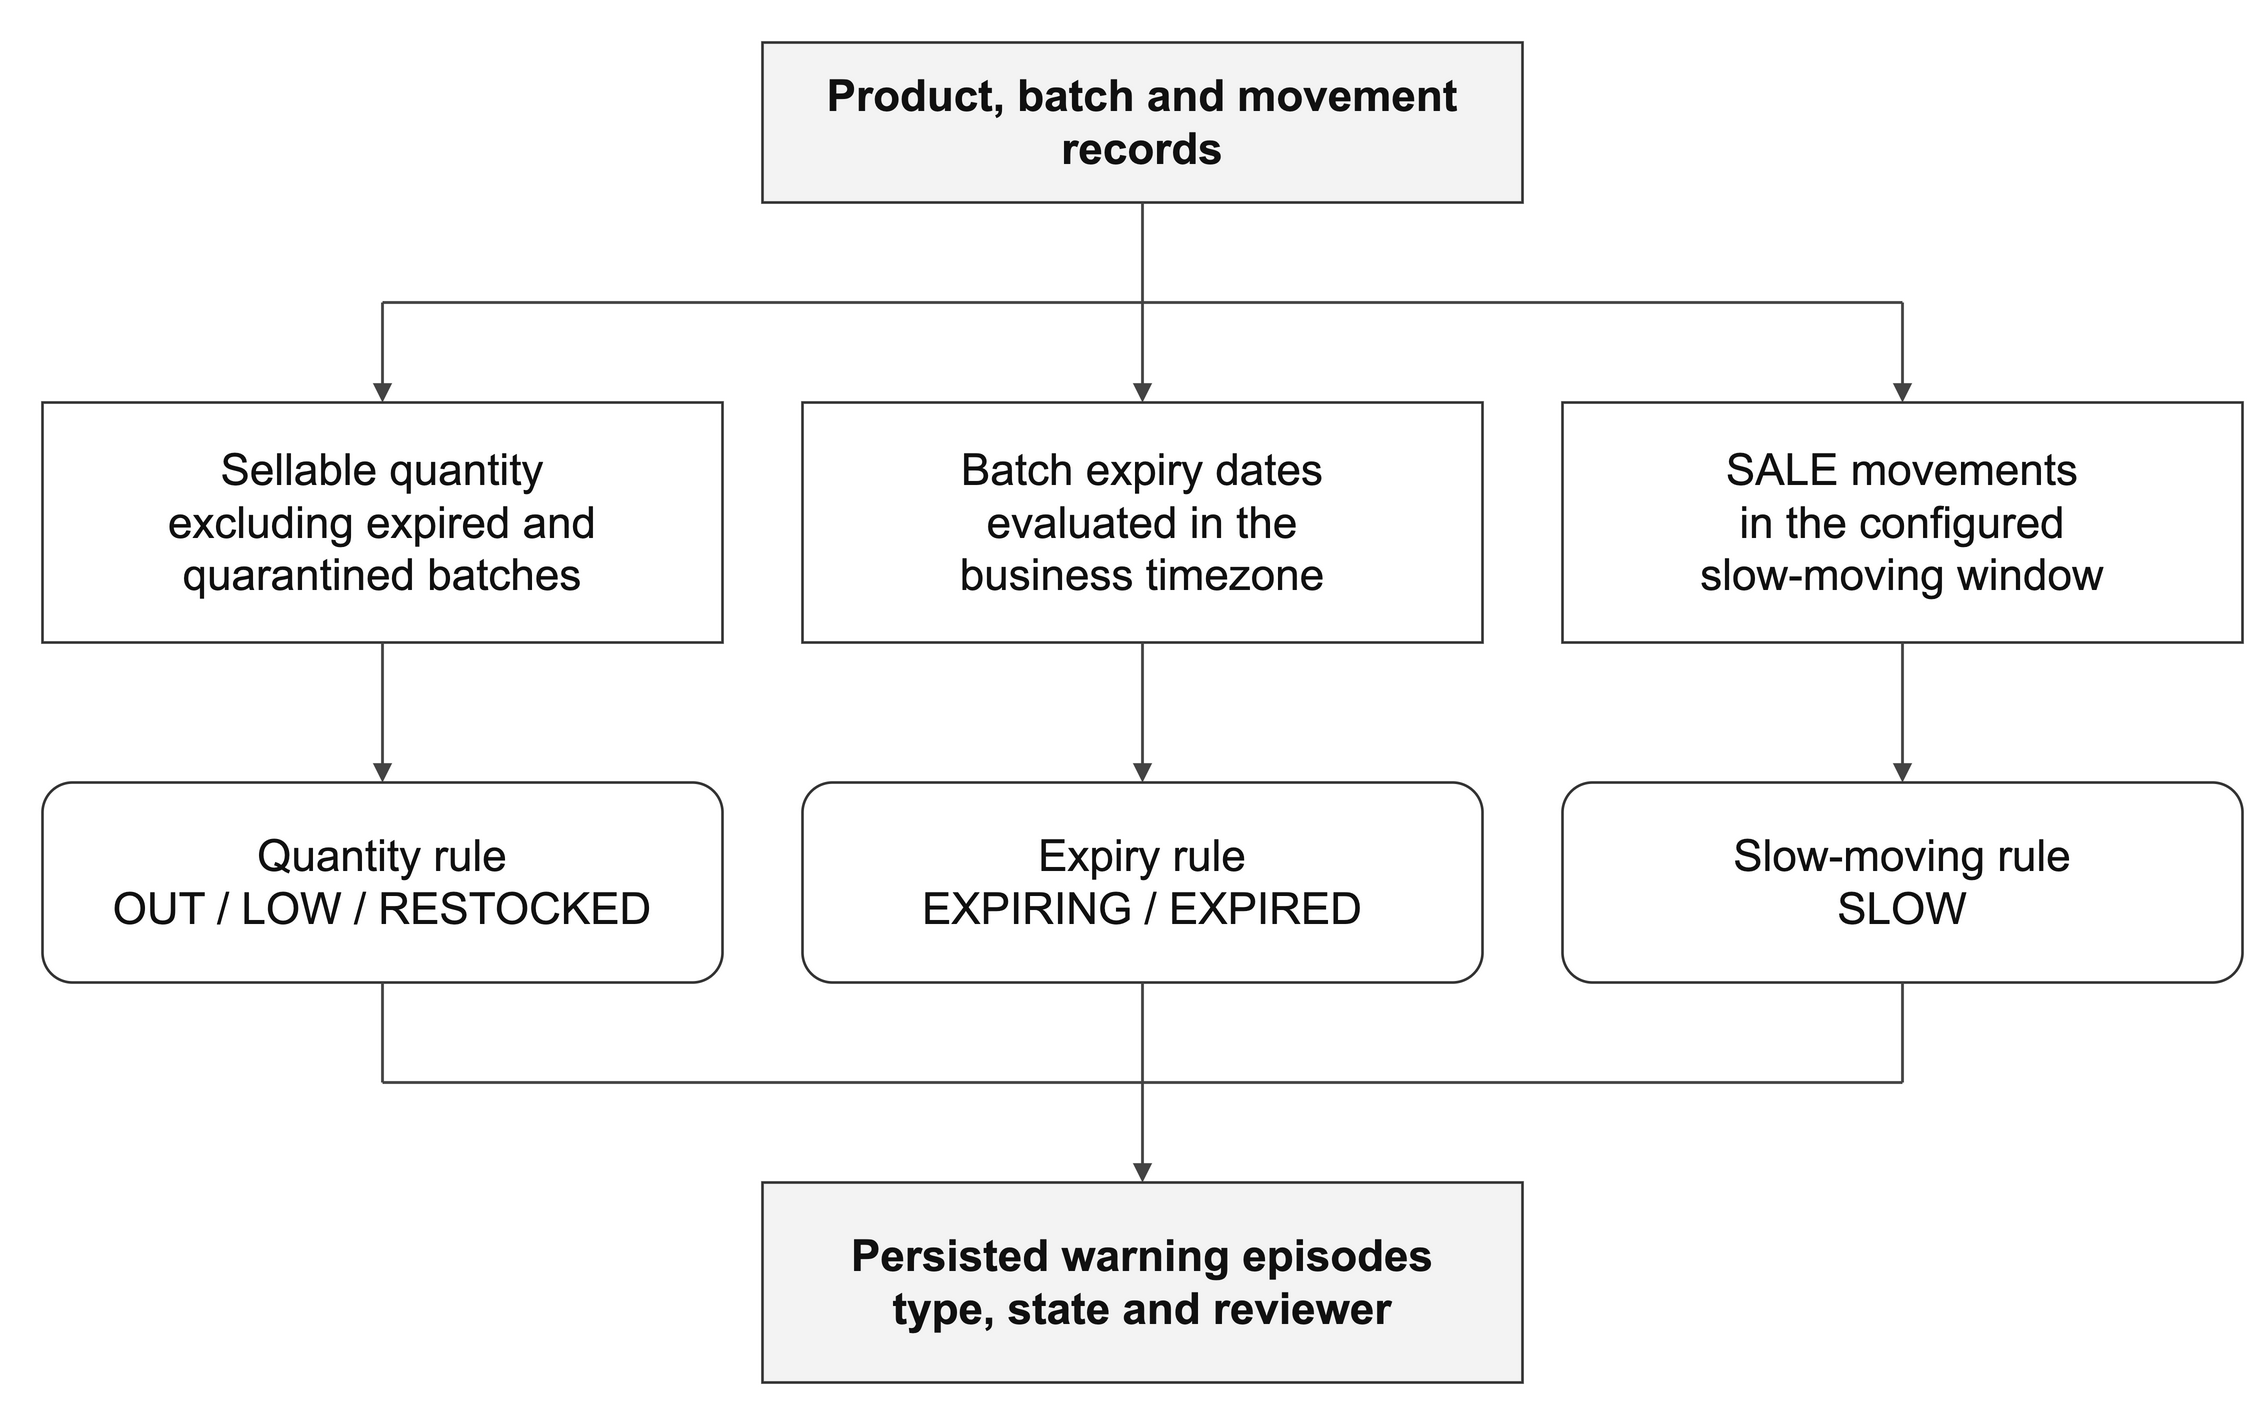
\includegraphics[width=\textwidth,height=0.70\textheight,keepaspectratio]{../figure-assets/diagrams/25-warning-rules.png}
\caption{Warning rule evaluation across batches, expiry, sales history and threshold policy}\label{fig:warning-rules}
\end{figure}

\subsection{Batch and purchasing objects}

A batch is the inventory identity created when a receipt carries production or expiry data, and physical and sellable quantities are maintained separately. FEFO selects the eligible batch with the earliest expiry date, and FIFO provides a deterministic order when dates are absent. Quarantine is an explicit control state that withdraws a batch from sale without erasing its movement history.


A replenishment suggestion compares sellable quantity plus the pending purchase position with the trigger threshold and target stock; it never creates an order on its own. A purchase document follows the states in Figure~\ref{fig:purchasing-workflow}. A draft is submitted and then approved or rejected; a rejected document can be edited back into a draft or resubmitted directly. Receipts against an approved document make it PARTIAL or COMPLETED, and any document that is not yet completed can be cancelled, which closes its remaining quantity. The document governs the internal purchasing decision and its inventory effects, while transmitting orders to suppliers remains outside the application.


\begin{figure}[htbp]\centering
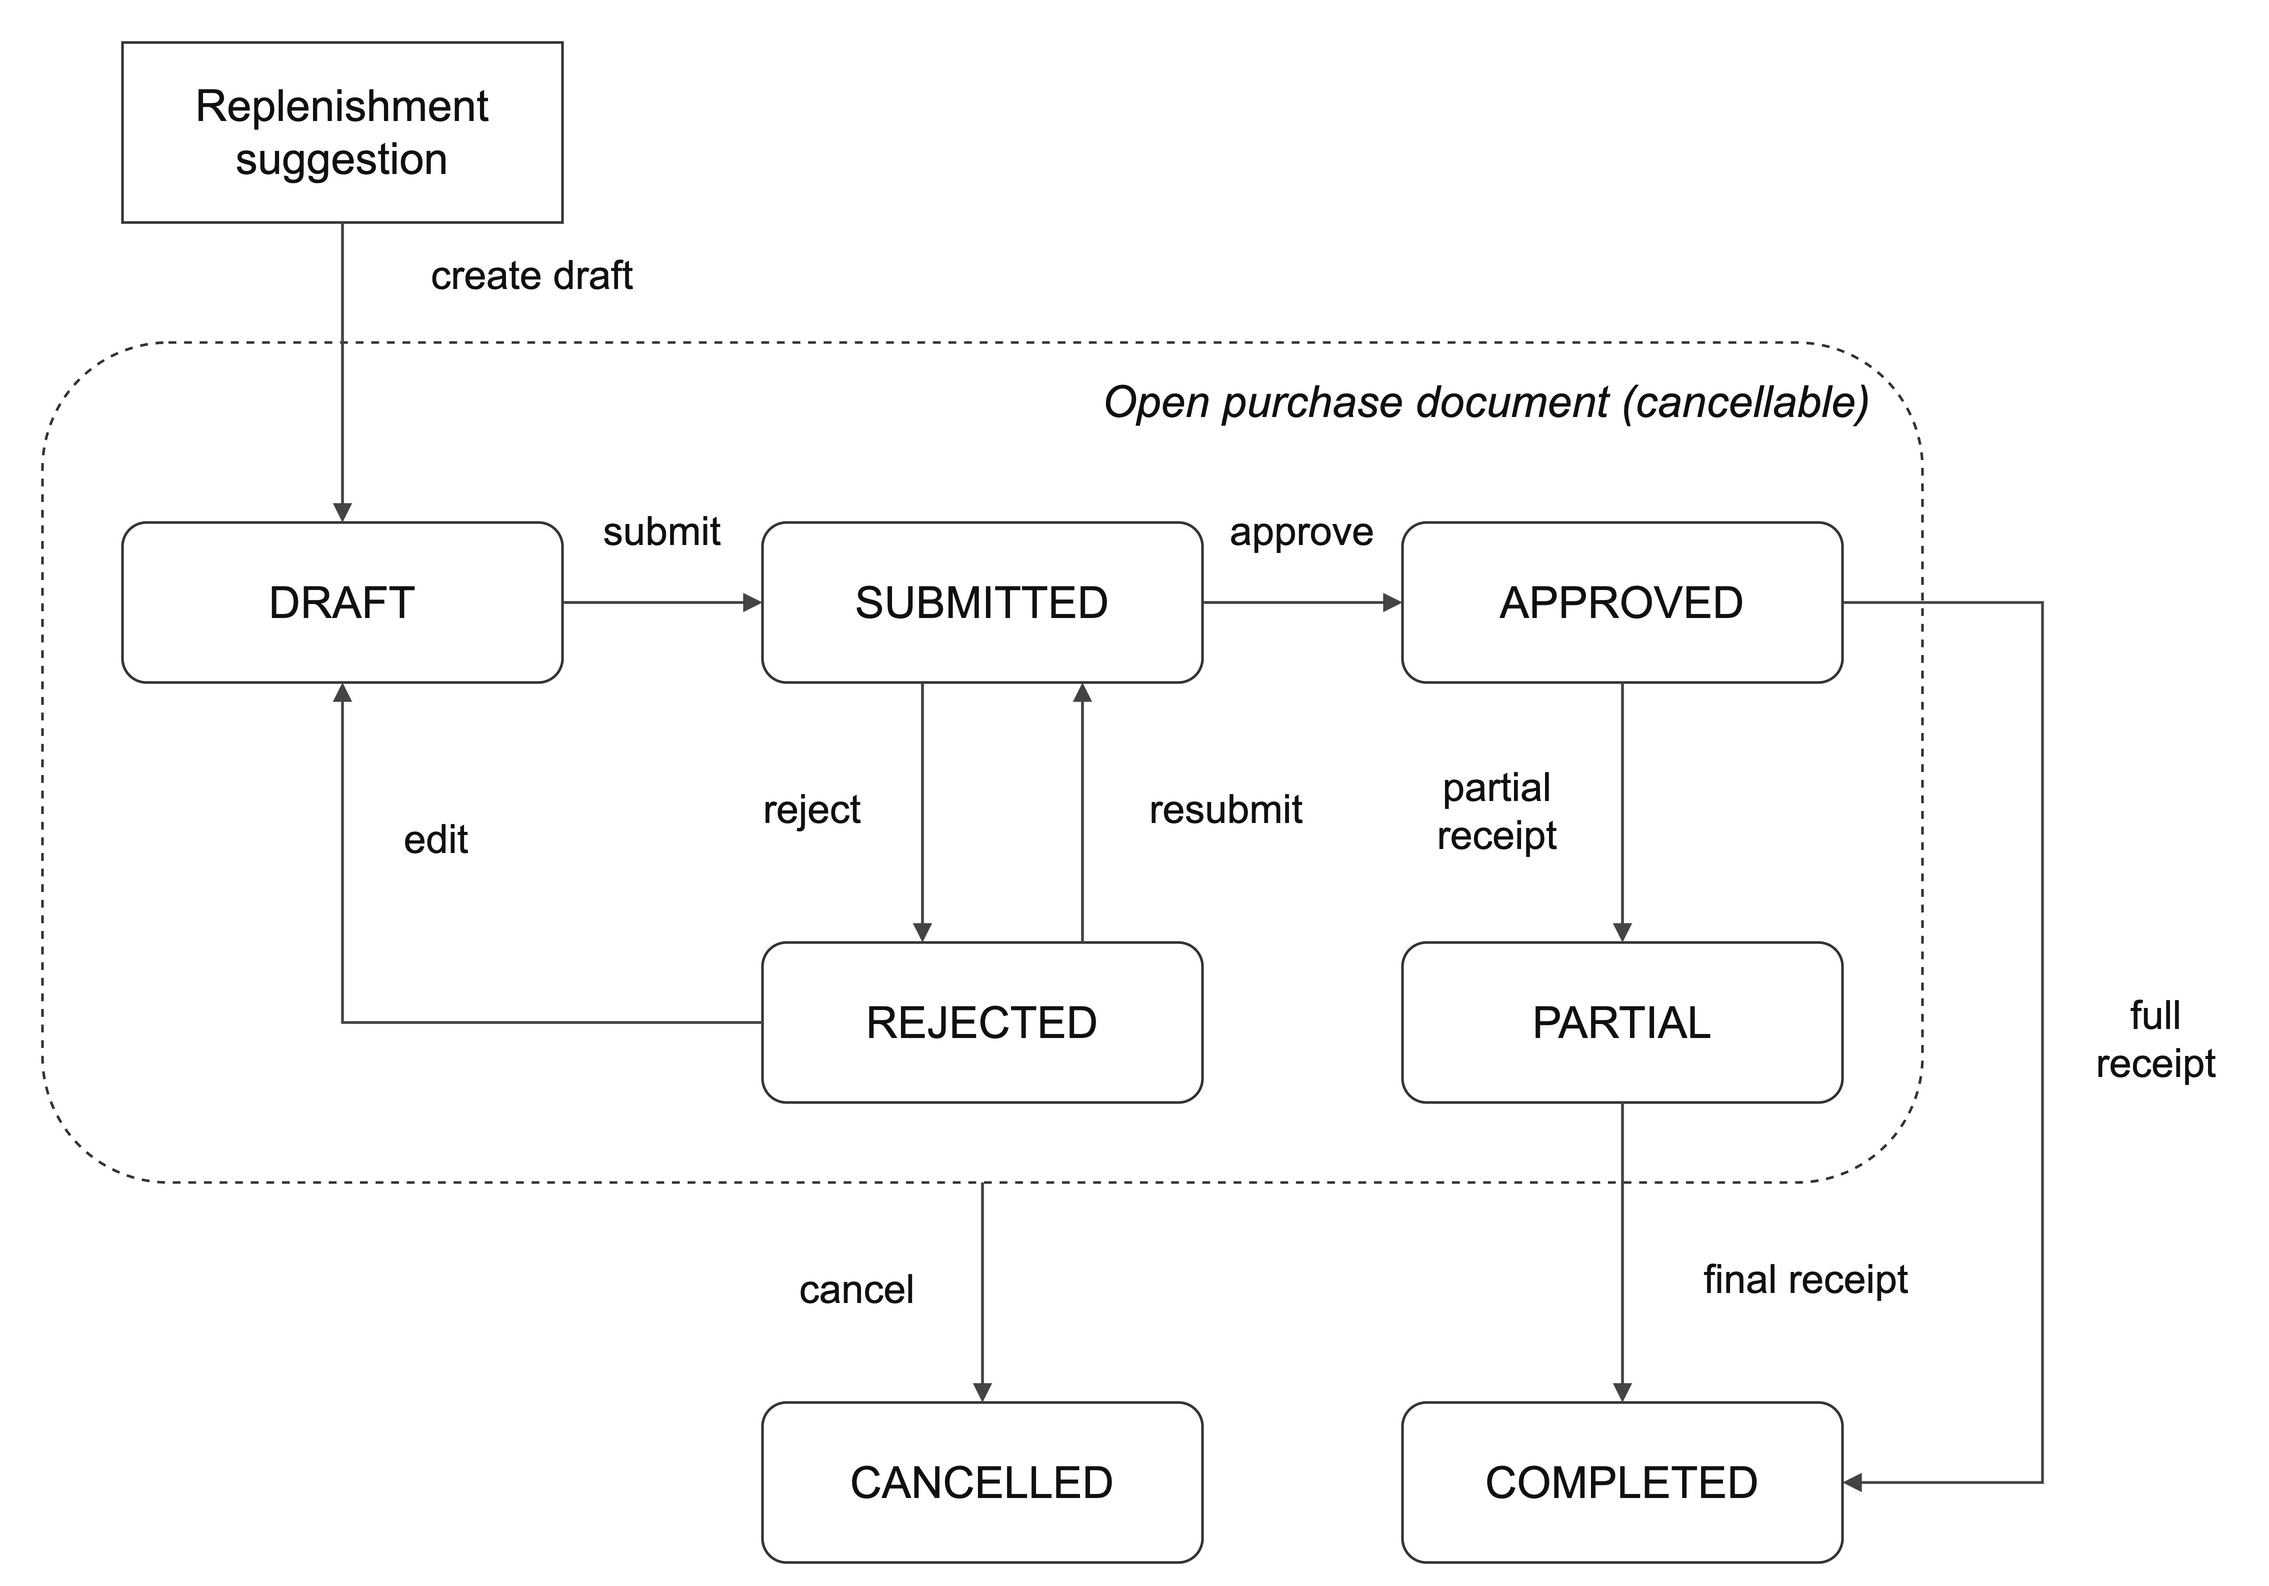
\includegraphics[width=\textwidth,height=0.70\textheight,keepaspectratio]{../figure-assets/diagrams/26-purchasing-workflow.png}
\caption{Replenishment suggestion through purchase approval and partial receipt}\label{fig:purchasing-workflow}
\end{figure}

A stock review records an intended count, adjustment or disposal against a quantity snapshot. Approval of a COUNT checks the product's quantity and version snapshot, approval of a DISPOSAL checks the remaining quantity of the selected batch, and an ADJUSTMENT applies its signed effect to the current locked balance. These checks prevent a delayed approval from overwriting a later receipt or dispatch.


\subsection{Reporting model}

Reports show active-product and shortage counts, the current-price value estimate, movement totals, recent activity and the category mix. The seven-day activity chart counts recorded movements by UTC date and is therefore not a sales chart, since receipts, adjustments and stocktakes also contribute. The category chart adds current unit counts, which is meaningful for the demonstration data but does not normalize different physical units.


The inventory CSV export contains the product page currently loaded. With twelve products per page, a large filtered selection may need several exports, each containing the fields visible on screen.


\subsection{Identity and administration model}

The application uses three fixed roles: ADMIN, MANAGER and CLERK. Each user has a username, display name, password hash, role, enabled flag and creation time. Administrators create users and change their access, while managers and clerks work within their assigned authority. Role changes and account suspension take effect on the next request, which limits reliance on authority cached in an old session.


At least one enabled administrator must always remain. This last-administrator guard prevents the store from losing access to staff administration. It complements rather than replaces authentication: a valid session still requires a currently enabled account whose role permits the requested action.


\FloatBarrier

\section{Domain invariants and representative scenarios}

The stock invariant combines arithmetic, bounds and attribution. The accepted after quantity equals the locked before quantity plus the derived delta, the balance and the movement record are written in the same transaction, and the quantity stays between zero and one billion. Product policy further requires a non-negative safety stock no greater than the reorder threshold. An invalid operation must leave both the balance and the history unchanged.


\begin{equation}q_{\mathrm{after}}=q_{\mathrm{before}}+\Delta,\qquad 0\leq q_{\mathrm{after}}\leq 10^9.\end{equation}

Consider a product with quantity seven and a reorder threshold of five. Dispatching two units leaves five and opens a LOW episode, because the threshold is inclusive. Dispatching the remaining five changes the severity to OUT. Acknowledging that episode records the review but leaves the quantity at zero. A later receipt of eight resolves the shortage and opens RESTOCKED. A subsequent count of three then yields a delta of minus five against the locked quantity of eight; it is not interpreted as adding three.


A retry is handled differently. Once an actor has recorded the count of three under a given key, resending the same normalized intention returns the earlier record, whereas a count of four under that key is rejected as a conflict. The rule of one intention per key thus links the business operation to the concurrency and retry design developed in Chapter 3.


\FloatBarrier

\section{Chapter summary}

The analysis identifies product balances, accepted movement history and warning episodes as the core consistency concepts, extended by batches, purchase documents and review snapshots. Chapter 2 turns these concepts into testable requirements.
